\chapter{General Introduction}

\section{Fruits and vegetable production challenges}

% Fruits and vegetables play an important role in human nutrition, as a source of trace elements, vitamins, and minerals. As the \gls{who} suggested for the healthy diet, at least 400 grams of them should be consumed per day to protect against malnutritions (\url{https://www.who.int/news-room/fact-sheets/detail/healthy-diet}). For example, broccoli (\textit{Brassica oleracea} L.) heads, one of the most important components of the global vegetable market, several case studies have demonstrated its great potential to prevent cancer and cardiovascular disease \citep{mahn_overview_2012,latte_health_2011}. However, their supplies and quality can be easily affected by extreme weather events (\url{https://www.bbc.com/news/business-64776969}). Moreover, climate change and global warming also have negative impacts on vegetables, especially lettuce and broccoli which need a cold accumulation period to produce a harvest \citep{bisbis_potential_2018}. In addition, different field management (e.g., tillage, density, and nutrient) also affects the vegetable yield and quality \citep{jackson_onfarm_2004, satodiya_effect_2015}. Hence, to ensure the vegetable supply and quality, it is important to monitor the plants during the growth stages and to take proper management decisions in time.

Fruits and vegetables are important sources of trace elements, vitamins, and minerals in human nutrition. The \gls{who} recommends consuming at least 400 grams of fruits and vegetables per day to prevent malnutrition (\url{https://www.who.int/news-room/fact-sheets/detail/healthy-diet}). For example, broccoli (\textit{Brassica oleracea} L.) heads, which are one of the most important components of the global vegetable market, have shown their great potential to prevent cancer and cardiovascular disease by several case studies \citep{mahn_overview_2012,latte_health_2011}. However, their supply and quality can be easily affected by extreme weather events (\url{https://www.bbc.com/news/business-64776969}). Moreover, climate change and global warming also have negative impacts on vegetables, especially lettuce and broccoli, which need a cold accumulation period to produce a harvest \citep{bisbis_potential_2018}. In addition, different field management practices (e.g., tillage, density, and nutrients) also affect vegetable yield and quality \citep{jackson_onfarm_2004, satodiya_effect_2015}. Hence, it is important to monitor the plants during their growth stages and make proper management decisions promptly to ensure vegetable supply and quality.

% Conventional agriculture management activities, like disease and pest monitoring and selective harvesting, requires heavy manual operations. Such artificial activities pose several challenges. First, judging the disease at the early stage and deciding whether proper harvest often require professional knowledge and can be subject to human errors. 
% Second, the available human labor in agriculture is decreasing nowadays. It is affected by both long-term global events like urbanization and aging population; and short-term pandemics like economic recession and \gls{covid19} \citep{gallardo_adoption_2018,larue_labor_2020}. Such labor shortage raises the labor costs and the costs will be passed on to the consumer end. In this scenario, labor-saving technologies have unprecedented demand. Combined with the fast development of technologies like automation, sensing, big data analysis, computer vision, and artificial intelligence, the agricultural industry has finally gone through the digital agriculture revolution \citep{gallardo_adoption_2018}.

Conventional agricultural management activities for such purposes require significant manual labor and are now facing several challenges. Firstly, they often require professional knowledge and may be subject to human error. Secondly, the availability of human labor in agriculture is currently decreasing due to long-term global events, such as urbanization and aging populations, as well as short-term pandemics, such as economic recessions and \gls{covid19} \citep{gallardo_adoption_2018, larue_labor_2020}. As a result, there is an unprecedented demand for labor-saving technologies. The development of technologies, such as automation, sensing, big data analysis, computer vision, and artificial intelligence, has made it possible to address such demands and thereby spark the digital revolution in the agricultural industry \citep{gallardo_adoption_2018}.

\section{Plant phenotyping techniques}
% background introduction for plant phenotyping
The labor-saving and digitized plant status monitoring, also named plant phenotyping, has been developed and implemented rapidly in recent years \citep{araus_field_2014}. It is defined as ``\textit{the application of methodologies and protocols to measure a specific trait related to plant structure or function with traits ranging from cellular to whole-plant levels}'' \citep{fiorani_future_2013, ghanem_physiological_2015}. Though different workflows are required for different crops and applications, the general workflow of plant phenotyping can be summarized as 1) Data collection, to collect plant or with background data by variate sensors; 2) \gls{roi} extraction, to detect or to segment plant parts at expected levels (e.g. full canopy or single organ) from the collected data; 3) crop traits calculation; and 4) practical or advanced applications.

\subsection{Data collection}
%% platform types -> indoor, outdoor(ground, aerial, satellite)
For the data collection, there are variable sensors for different plant phenotyping purposes. The sensors can be split into environmental sensors (e.g. light intensity, temperature, and humidity) and plant sensors (e.g. organic compounds, plant images) \citep{garlando_plants_2020}. The environmental sensors are often set in a fixed place, as an important component of \gls{iot}, to record environmental factors which are crucial and can affect plant phenotypes \citep{ghanem_physiological_2015}. While plant sensors are often set on and moved with the platforms (Fig.~\ref{fig:int1}). From the indoor (Fig.~\ref{fig:int1}a-d)to the outdoo (Fig.~\ref{fig:int1}e-k), the scale of collected data using these platforms also changes from organ level, individual level to canopy level.

\begin{figure}[htb!]
  \begin{center}
    \resizebox{\textwidth}{!}{
      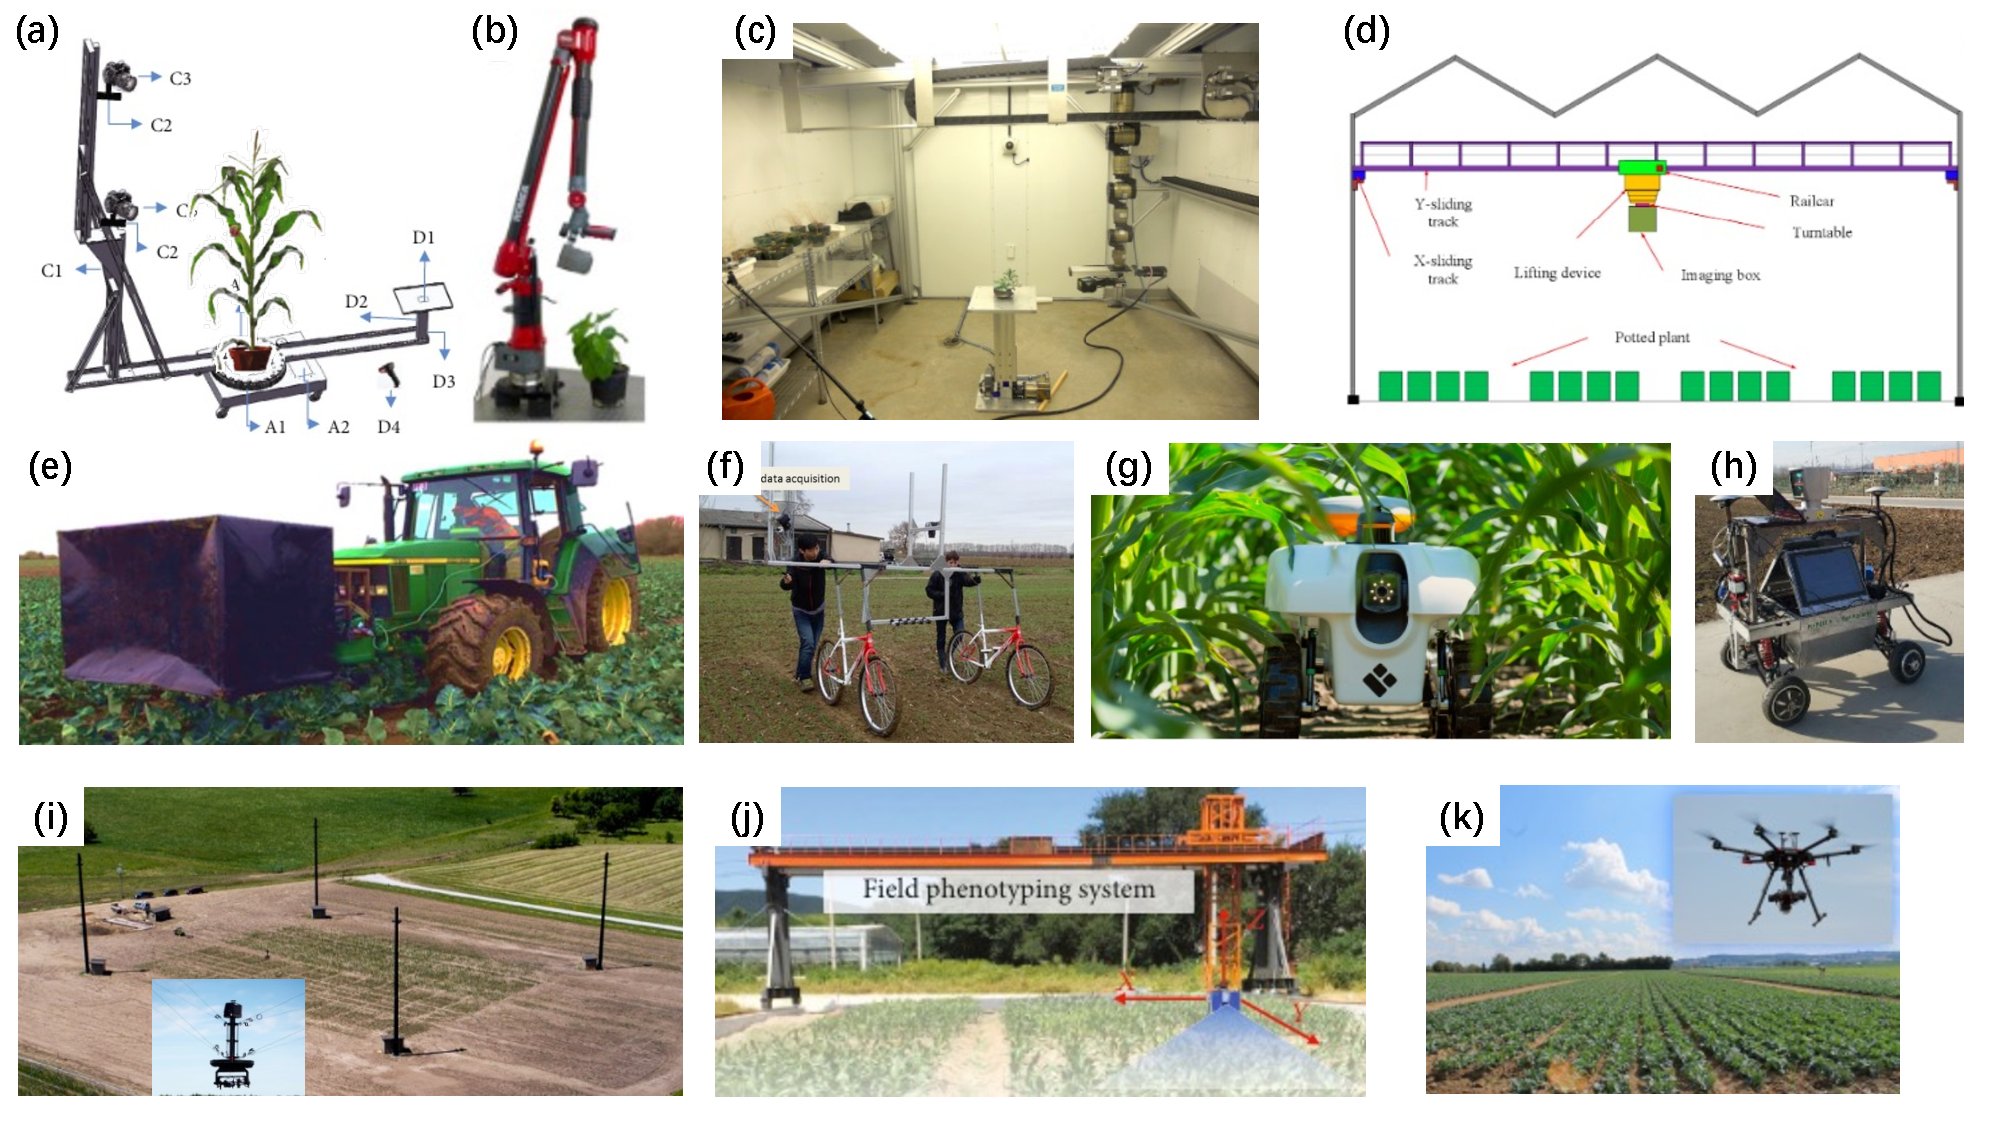
\includegraphics{figures/int/platforms.pdf}
    }
  \end{center}
  \caption[Example of platforms for plant phenotyping]{
    Example of platforms for plant phenotyping. (a-b) self-designed indoor devices \citep{wu_mvs-pheno_2020,schunck_pheno4d_2021}; (c-d) robotic arms in growth chamber or greenhouse \citep{chaudhury_machine_2018, du_greenhouse_2021}; (e) tractor \citep{kusumam_3d_2017}; (f) ground vehicle \citep{liu_estimation_2017}; (g-h) \gls{ugv} \citep{mcguire_high_2021, qiu_field-based_2019}; (i-j) robotic outdoor instruments \citep{bai_nu-spidercam_2019, jin_exploring_2021}; and (k) \gls{uav} \citep{kierdorf_growliflower_2022}
  }
  \label{fig:int1}
\end{figure}

% From the indoor to the outdoor, the commonly used platforms include self-designed indoor devices \citep{wu_mvs-pheno_2020,schunck_pheno4d_2021}, robotic arms in growth chamber or greenhouse \citep{chaudhury_machine_2018, du_greenhouse_2021}, tractor \citep{kusumam_3d_2017,blok_effect_2021}, ground vehicle \citep{liu_estimation_2017}, \gls{ugv} \citep{mcguire_high_2021,qiu_field-based_2019}, robotic outdoor instruments \citep{bai_nu-spidercam_2019, jin_exploring_2021}, \gls{uav} \citep{kierdorf_growliflower_2022, jang_review_2020}, and even satellite \citep{nguyen_monitoring_2020}. The scale of collected data using these platforms also changes from organ level, individual level to canopy level.


An important part of plant sensors is imaging sensors, which can record the morphological information of crops and are therefore commonly used in many plant phenotyping studies \citep{paulus_measuring_2019, feng_comprehensive_2021}. For example, the infrared, multi- and hyper-spectral imaging sensors were used to calculate several vegetation indices \citep{han_modeling_2019}, like \gls{ndvi}, to assess biomass \citep{jimenez-berni_high_2018}, yield and water stress level \citep{, herrero_yield_2020, romano_use_2011}, and broccoli head freshness \citep{guo_evaluation_2022}. The common \gls{rgb} camera was also used to count plant number \citep{liu_estimating_2022}, plant density \citep{velumani_estimates_2021}, detect the broccoli head \citep{blok_machine_2016}, and access broccoli head quality \citep{stansell_use_2017}. They show the feasibility of imaging sensors in plant phenotyping with great efficiency and non-destructive dependency.

%% 3D sensors
% introduction for 3D phenotyping, method to obtain 3D (passive, active) -> cost limit, choose RGB+SfM
However, these approaches are hard to describe the 3D morphological structure of plants due to occlusion and dimension loss when projecting onto the 2D plane. As a result, it produces inaccuracies and uncertainties for 3D phenotyping applications. With the development of sensing techniques, several studies reviewed available approaches for the 3D plant phenotyping \citep{paulus_measuring_2019, okura_3d_2022, kochi_introduction_2021}. Figure~\ref{fig:int2} summarizes some of them which are mostly used.

\begin{figure}[htb!]
  \begin{center}
    \resizebox{\textwidth}{!}{
      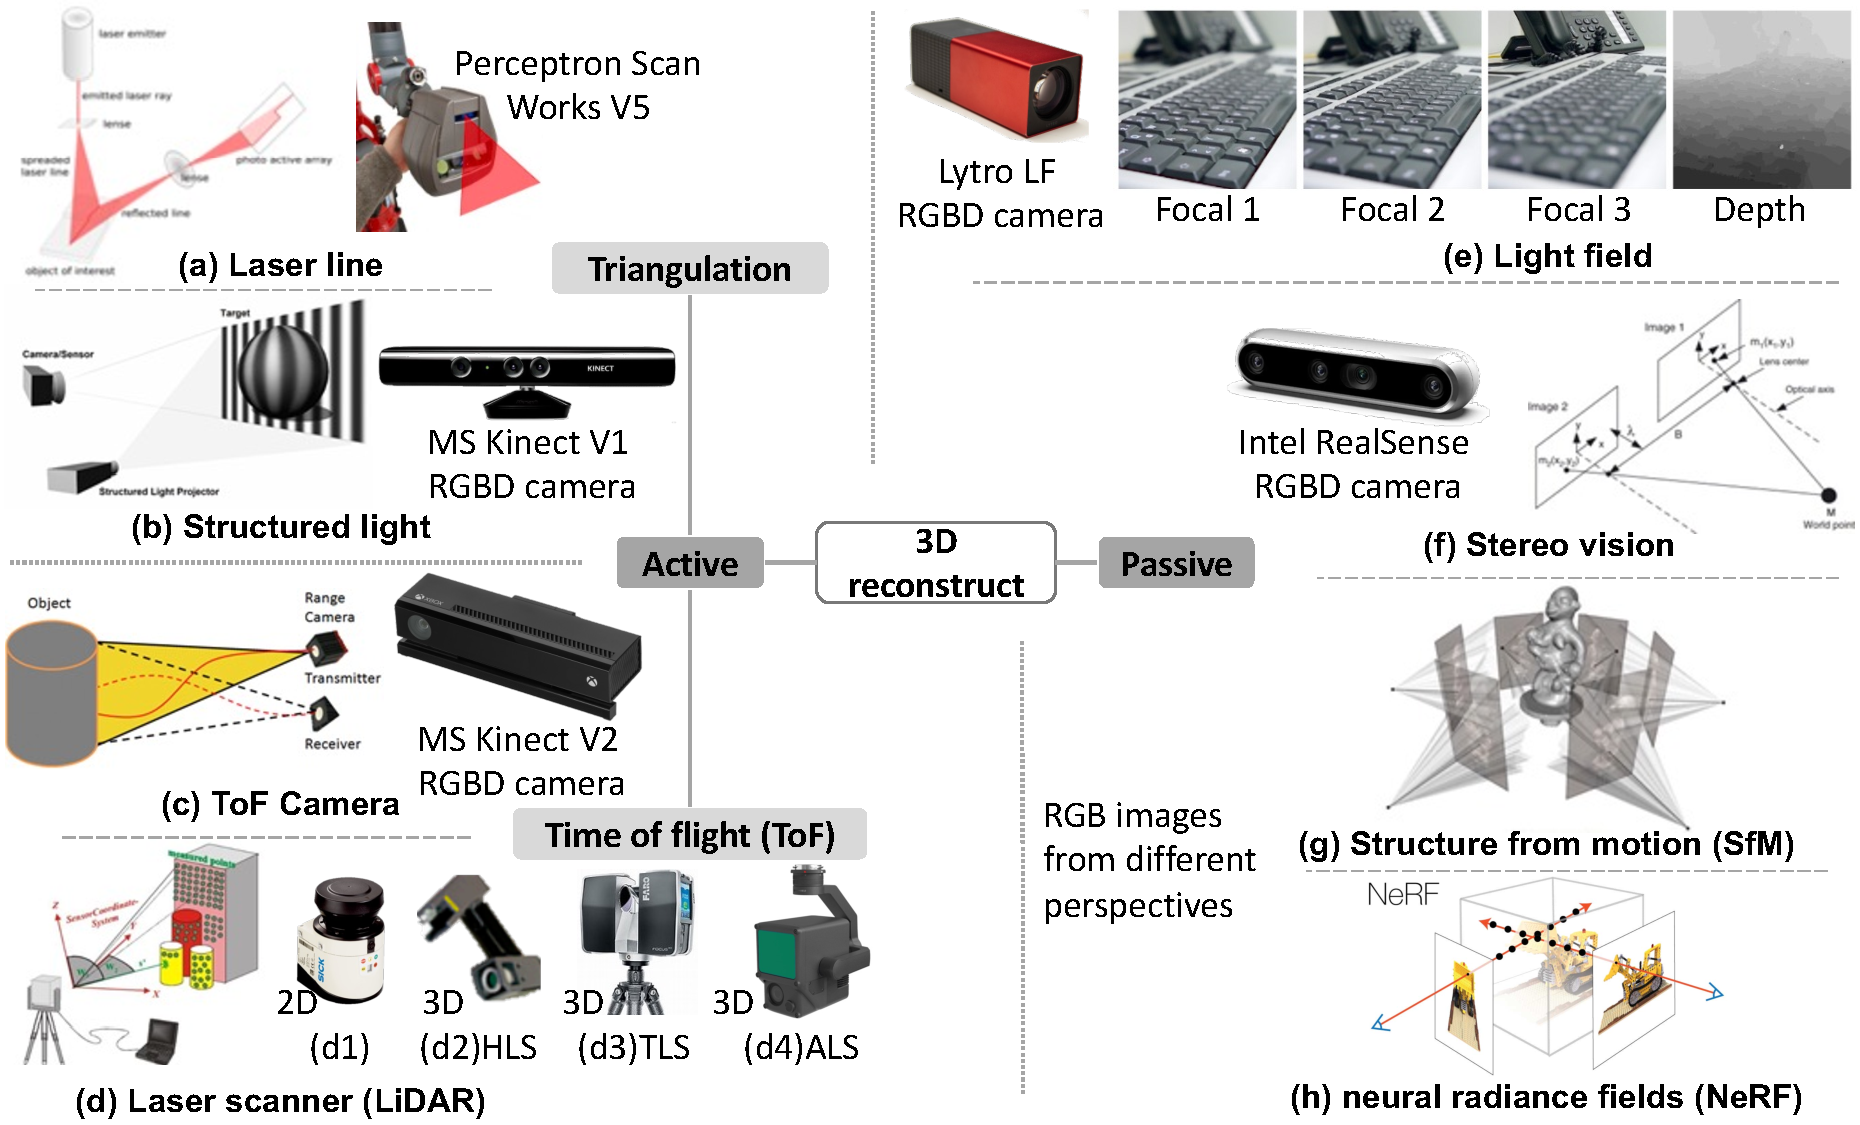
\includegraphics{figures/int/recons_sensors.pdf}
    }
  \end{center}
  \caption[Common methods for 3D structure reconstruction]{
    Common methods for 3D structure reconstruction. (a-d) The active sensors rely on projecting lights on the object and analyzing the reflection results, where (d) \acrfull{lidar}; (d2) \acrfull{hls}; (d3) \acrfull{tls}; (d4) \acrfull{als}; (e-g) the passive sensors rely on analyzing the passively received image groups. 
  }
  \label{fig:int2}
\end{figure}

% Realsense用的Stero Camera没问题,但是Kinect v1是基于红外线的形变,kinectv2是红外线的ToF
% but it seems Kinect V1 uses infrared structured light and Kinect V2 uses the infrared time-of-flight.

The active sensors rely on projecting and receiving the reflections from the object. The triangulation uses the shape changes on the projected straight laser line(s) to obtain the object structure. The time of flight measures the distance between the sensor and points on the object to obtain the structure. While the passive sensors rely on analyzing the passively received images. The light field camera takes a group of photos with different focal lengths, the shape of object is calculated according to different degrees of clarity caused by the different distances to the sensor. The structure from motion uses the overlapped area among images to estimate the camera poses and object structure. The stereo uses known binocular disparity to obtain structure of object.



%% software SfM

%% sfm in agricultrual applications.

% \subsection{Data analysis for phenotyping}
% for data analysis.

\subsection{ROI extraction}

\subsubsection{Image analysis}
%% image analysis

%%% traditional CV method

%%% deep learning based method

\subsubsection{3D analysis}
%% 3D data analysis

%%% remove background

%%% segmentation

%%%% individual segmentation

%%%% organ segmentation

\subsection{Traits calculation}
% du_greenhouse_2021 -> 100多个参数

%% 1D 参数

%% 2D 参数

%% 3D 参数

\subsection{Advanced application}

%% 收期预测、光照模拟

\section{Challenges in plant phenotyping}



\section{Objective of this study}

\begin{enumerate}
    \item To develop an almost-automatic 3D reconstruction workflow that can obtain the integrate and high-quality 3D models of destructively sampled broccoli heads.
    \item To develop an unsupervised phenotyping workflow that can automatically segment the broccoli crown part from Objective 1, and calculate several 1D to 3D morphological traits.
    \item To develop an improved workflow for \gls{uav}-based 3D reconstruction broccoli canopy using the 3D to 2D projection and labor-saving deep learning technique, which can obtain better 2D morphological traits of broccoli heads in complex outdoor conditions.
    \item To combine the strengths of the \gls{uav}-based pipeline (high throughput but low quality) and the destructive-based pipeline (high quality but low throughput). Using the auto machine learning regression and the template matching to recover the 3D traits from \gls{uav}-based 2D traits for all broccolis in the field.

\end{enumerate}


\section{Outline of this study}

Chapter 1 is an overview of the study's background information, relative studies, and objectives

Chapter 2 develops and validates the 3D phenotyping pipeline for destructively sampled broccoli heads using the photogrammetry technique, which includes obtaining high-quality plant 3D models and calculating the 3D traits.


Chapter 3 develops and validates the 3D phenotyping pipeline for \gls{uav} sensing on broccoli canopy, includes the 3D to 2D projection pipeline to improve deep-learning-based phenotyping

Chapter 4 tests the idea of cross-scale assimilation of broccoli based on the pipeline built in Chapter 2 and Chapter 3.

Chapter 5 summarizes the general conclusions of this study, and also discusses the research prospects in the future.